\documentclass[12pt,twoside,openright]{report}
\usepackage{svniteced_thesis}
%%\renewcommand{\baselinestretch}{1}
\usepackage{cuted}
\usepackage{graphics}
\usepackage{graphicx}
\usepackage{amsmath}
%\usepackage{amssymb}
\usepackage{color}
\usepackage{csquotes}
\usepackage[dvipsnames]{xcolor}
\usepackage{epstopdf}
\usepackage[T1]{fontenc}
\usepackage[utf8]{inputenc}
\usepackage{multirow}
\usepackage{subfigure}
\usepackage{float}
\usepackage{amsmath}
\usepackage{array}
\usepackage{algorithm}
\usepackage{algorithmic}
\usepackage{verbatim}
\newcommand{\RNum}[1]{\uppercase\expandafter{\romannumeral #1\relax}}
\usepackage{tabularx}
\usepackage{times}
\usepackage{fancyhdr}
\usepackage{rotating}
%\usepackage{fancyheadings}
\usepackage{footnote}
\usepackage{morefloats}
\usepackage{amsfonts}
\usepackage{amssymb}
\usepackage{type1cm}
\usepackage{eso-pic}
\usepackage{fancybox}
\usepackage{lipsum}
\usepackage{geometry}
\usepackage{makeidx}
\usepackage[justification=centering]{caption}
\usepackage{wrapfig}
\usepackage{afterpage}
\usepackage{lscape}
\usepackage{longtable}
%\usepackage{cite}
\usepackage{float}
\usepackage{amsmath}
\usepackage{hyperref}
\usepackage{multirow}
\usepackage[numbers]{natbib}
\usepackage{notoccite}
\usepackage{enumerate}
\usepackage{placeins}
\usepackage{rotating}
\usepackage{setspace}
\usepackage{lipsum}
\usepackage{titlesec}
\titlespacing\section{0pt}{12pt plus 4pt minus 2pt}{0pt plus 2pt minus 2pt}
\titlespacing\subsection{0pt}{12pt plus 4pt minus 2pt}{0pt plus 2pt minus 2pt}
\titlespacing\subsubsection{0pt}{12pt plus 4pt minus 2pt}{0pt plus 2pt minus 2pt}

\begin{document}
%%%%%%%%%%%%%%%%%%%%%%%%%%%%%%%%%%%%%%%%%%%%%%%%%%
% Title of the Project
\title{Dissertation Title}
\Degree{Master of Technology}
\Specialization{VLSI \& Embedded Systems}
\AcadYear{2020-21}
%%%%%%%%%%
\author{Student Name}
\AdmNo{Roll Number}
%%%%%%%%%%
%For example
\GuideName{Prof. AAAAAA}						
\GuidePos{Associate Professor}
\GuideAssociation{ECED-SVNIT}							%\GuideAssociation{ECED}

% If there is Co-Guide, please enter the following fields.
% If there is no Co-Guide, either comment the lines or delete them. Don't leave them blank.
\CoGuideName{Dr. BBBBBB}
\CoGuidePosn{Assistant Professor}
\CoGuideAssociation{ECED-SVNIT}
%
\ExaminerName{Dr. XXX}
\ChaimanName{Dr. ZZZ}

%\date{2020-21}
\date{July 2021}
%%%%%%%%%%%%%%%%%%%%%%%%%%%%%%%%%%%%%%%%%%%%%%%%%%
\MakeTitlePage
\MakeCerti
%%%%%%%%%%%%%%%%%%%%%%%%
\pagestyle{plain}
\pagenumbering{roman}
%\newpage
\clearemptydoublepage
%%%%%%%%%%%%%%%%%%%%%%%%
% acknowl.tex {Acknowledgements}

\chapter*{Acknowledgements}
%write your acknowledgements here
\begin{flushright}
	\author\\
	Student name\\[0.01in]
	Roll number\\
	Sardar Vallabhbhai National Institute of Technology\\
	Surat\\
	Date:  30 / 11/ 2019\\
\end{flushright}



\addcontentsline{toc}{chapter}{\textbf{Acknowledgement}}
%%%%%%%%%%%%%%%%%%%%%%%%
\cleardoublepage
%\Acknowledgement{acknowl}
\Abstract{abstract}
%%%%%%%%%%%%%%%%%%%%%%%%
% Declaration Page

%\addcontentsline{toc}{chapter}{\textbf{Declaration}}

\chapter*{Declaration}

I declare that this written submission represents my ideas in my own words and where others' ideas or words have been included, I have adequately cited and referenced the original sources. I also declare that I have adhered to all principles of academic honesty and integrity and have not misrepresented or fabricated or falsified any idea or data or fact or source in my submission. I understand that any violation of the above will be cause for disciplinary action by the Institute and can also evoke penal action from the sources which have thus not been properly cited or from whom proper permission has not been taken when needed.\\
\\
\\
\\
\begin{minipage}[t]{7cm}
	\begin{flushleft}
			\vspace*{7mm}
		Date:02/12/2019.\\
		Place:Surat.\\
	\end{flushleft}
\end{minipage}
\hfill
\begin{minipage}[t]{7cm}
	\begin{flushright}
		%	\vspace{0.5cm}
		\line(1,0){100}\\
		Anegondi Krishnama Raju\\[0.01in]
		(P18EC011)\\
		%	\vspace{0.5cm}
	\end{flushright}
\end{minipage}

\addcontentsline{toc}{chapter}{\textbf{Declaration}}
%%%%%%%%%%%%%%%%%%%%%%%%
\TableOfContents
\ListOfFigures
%\ListOftables
\listoftables
%\newpage
\cleardoublepage
%\clearemptydoublepage
%%%%%%%%%%%%%%%%%%%%%%%%
%%\chapter*{List of Acronyms}
\begin{center}
  \textbf{\LARGE{List of Acronyms}}
\end{center}
\vspace{2pt}
\begin{longtable}{ll}


EFPI & Extrinsic Febry Perot Interferometry \\
FDA & U.S Food and Drug Administration\\ 
FFT & Fast Fourier Transform \\
FSR & Free Spectral Range \\
MMF & Multi Mode Fiber \\
MSE & Mean Square Error \\
RIU & Refractive Index Unit \\
SMF & Single Mode Fiber  \\


%   &  \\
\end{longtable}
%\newpage
%\thispagestyle{empty}
%\mbox{} 
%\addcontentsline{toc}{chapter}{\textbf{Abbreviations}}
%%%%%%%%%%%%%%%%%%%%%%%%
%\newpage
%\input{listofsymbols}
%\addcontentsline{toc}{chapter}{\textbf{List of Symbols}}
%%%%%%%%%%%%%%%%%%%%%%%%
\StartBody
\doublespacing
\pagestyle{fancy}
\begin{chapter}{Name of chapter 1}
\setcounter{secnumdepth}{4}
\label{chap:chap1}
%write your chapter content here
%for example visit chapter 2 and chapter 3
\section{name of section}
Currently wireless \citep{gha} technology finds its widest expression in fixed and mobile roles. In the fixed role, wireless is used extensively for data transfer, especially from desktop computers and lap-tops. In the mobile role, wireless networks provide mobility for use from fast vehicles for both voice and data. A base station (BS) with 100s or even 1000s of antennas we will provide in a centralized or distributed manner, such a integrated system can potentially reduce multiuser interference along with provide a multi fold increase in cell data throughput \cite{wen}. \\
\end{chapter}

\begin{chapter}{Name of chapter}
\setcounter{secnumdepth}{2}
\label{chap:chap2}

%write your chapter content here
\section{name of section}
\textbf{Title: OFDM channel estimation by singular value decomposition \cite{edf}[1998]}\\
 
\section{summary}
%\begin{center}
%\begin{longtable}{ | m{2cm} | m{3cm} | m{9cm} |} 
%\hline
%\textbf{year} & \textbf{Authors} & \textbf{Remarks}\\ \hline
%1988  & Edfors et.al \cite{edf}  &used low channel estimators for ofdm channel estimation using frequency correlation of channnel. Used 16-QAM evaluated performance of system in symbol error rate(SER)  \\ 
%\hline
%2007  & Musolino et.al \cite{mus} & a new adaptive identification method for  blind power-line channel estimation and equalization for OFDM communication systems.whenever channel has more nonlinearities proposed method works well \\
%\hline
%2012 & C Chen, MD Zoltowski et.al \cite{vari} & Given analysis of  sparse channel estimation for OFDM based on basian learning  and larger time delay  estimation of the doubly selective channel in a multiple consecutive OFDM symbols will be avoided \\
%\hline
%2012 & F Li, Z Xu, S Zhu et.al \cite{liva} & proposed methods are useful in combat imperfect channel estimation at the receiver side and  low-complex detection techniques based on variational inference proposed for channel estimation  \\
%\hline
%2017&S Dörner, S Cammerer, J Hoydis \cite{dor} &End-To-End Communication systems blocks will be replaced by trained Neural Networks, performance can be restricted by receiver synchronization and short block lenghts, First time hyper parameter tunning is propsed for increasing efficiency of Nural networks. \\
%\hline
%2018 & FA Aoudia, J Hoydis et.al \cite{aou} &Reinforcement based training for transmitter, Supervised training for receiver, prior knowledge of channel conditions are not needed, Requires additional feedback channel during the training to compensate the feed back losses from receiver to transmiter.\\
%\hline
%\endfirsthead
%\hline
% \textbf{year} & \textbf{Authors} & \textbf{Remarks}\\ \hline
% 2019& M Soltani, V Pourahmadi, A Mirzae et.al \cite{solt} & Time frequency channel grid of considered as two-dimensional image which knows it values only at pilot positions. This will be treated as low resolution image(LR) and channel estimated will be considered as high resolution(HR) image. Image Super resolution(SR) algorithm will be applied for converting LR image to HR image.\\
% \hline
% 2019& Z Qin, H Ye, GY Li, BHF Juang et.al \cite{qinp} & Joint channel estimation and detection is proposed, 5-layer fully connected DNN model  into OFDM receiver considering channel as block box, channel estimation is done by internally here DNN model so it can recover the transmitted data without estimating CSI externally.\\ \hline
%%\caption{Summary of Literature reviews.\label{long}}\\
%\end{longtable}
%\end{center}





\begin{center}
     ***
 \end{center}



















\end{chapter}
\chapter{Name of chapter 3}
\setcounter{secnumdepth}{3}
\label{chap:chap3}
\section{Overview}

Orthogonal frequency Division Multiplexing (OFDM) employs Multi-Carrier Modulation (MCM) technique highly attractive for implementation and received considerable attention due to the need for high speed data transmission. Orthogonal sub carriers allow their spectrums to overlap which achieves the high spectral efficiency.



\section{Hyperparameter Tunning-Improving neural networks}
Building a Deep neural network architecture for a specific application it is not a big issue. To reduce the time needed for training deep neural network model and for improving its accuracy we have to use hyperparameter tuning. These techniques are very useful for reducing training period. This section divided into three parts i.e first part will explain how to divide the data into training set, development set, test set and it covers some regularization techniques, dropout methods, batch normalisation process etc. Part 2 will give brief idea about optimizers that is RMSprop and Adam optimizer. Finally we can see how hyperparameter tuning can improve the model efficiency. Choosing hyperparameters and observing their effect on efficiency it is very crucial part in training neural networks. There is no standardized way for choosing hyperparameters. We can select hyperparameters according to the results given by tuning this is completely observation process.\\
\par Some of the hyper parameters are listed below 
\begin{itemize}
    \item Different types of active functions used at input, hidden  and output layers. 
    \item  Learning rate 
    \item How many hidden layers and how many units present in each hidden layer.
\end{itemize}


\subsection{Bias and Variance}
If we are classifying objects using a straight line then and it is called under-fit and it is highly biased. If we will classify the objects perfectly using curves then it is called over-fit and that are high variance. 

\begin{figure}
    \centering
    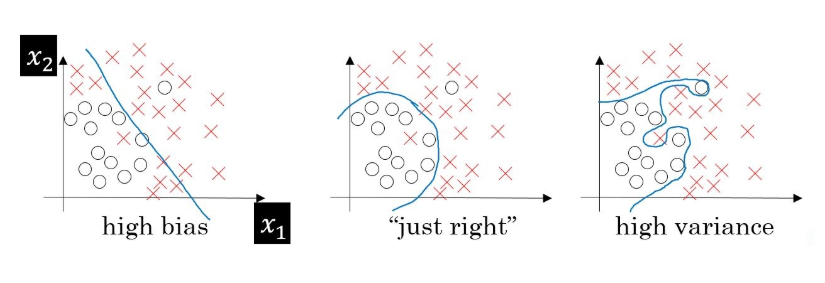
\includegraphics[width=15cm,,scale=5]{Screenshot (137).png}
    \caption{ Curves for showing under fit and over fit data \cite{jain} }
    \label{fig:my_label}
\end{figure}

For best model always bias and variance values should be less. Choosing the best model includes checking the training set and testing set error. 
some points to keep in mind for choosing the model 


\begin{itemize}
    \item If test set error is greater than train set error then model representing over fitting and it has high variance.
    \item If test set and train set error both are having high value then model represented as underfitting and it has high bias.
    \item  If Training set error is more than test set error then model has high variance and high bias. 
    \item  Train set and test set error both are small then data is fitted reasonably, Hence model as low variance and low bias.
\end{itemize}




\begin{center}
     ***
 \end{center}




%%%%%%%%%%%%%%%%%%%%%%%%
\StartRef
\include{bib}
\bibliographystyle{IEEEtran}
%\bibliography{IEEEabrv}
\bibliography{bibliograph}
%%%%%%%%%%%%%%%%%%%%%%%%
% If you have more than one Appaendices use
% '\StartAppendices' instead of '\StartAppendix'
%\StartAppendix			% 'Appendix' will be printed in Table of Contents
%\StartAppendices		% 'Appendices' will be printed in Table of Contents
%\Appendix{Appendices/AppendixA}
%\Appendix{Appendices/AppendixB}
\end{document}
